\chapter{Resultados}   
\minitoc

\section{Comparaci\'on de propiedades \'opticas entre sistemas moleculares dipolar, cuadrupolar y octopolar}

Inicialmente se prepararon soluciones en THF y suspensiones acuosas de nanopart\'iculas para las mol\'eculas 1NDS, 2NQS y 3NOS (Ver Figura \ref{ar2}) a una concentraci\'on de $6.25 \times 10^{-6}$ utilizando CTAB. En la figura \ref{X} se muestran los espectros de absorci\'on lineal molar $\epsilon$ de estas soluciones y suspensiones. La mayor absorci\'on se presenta en el sistema octopolar, posteriormente en el sistema cuadrupolar y finalmente en el sistema dipolar. 

\begin{figure}[h]
\centering
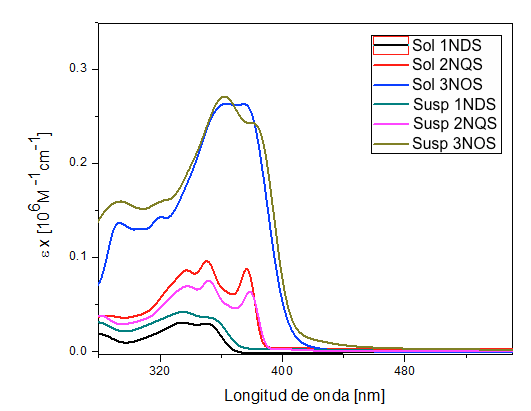
\includegraphics[width=0.85\textwidth]{resultados/sec1/comp}
\caption{Espectros de absorci\'on molar de 1NDS, 2NQS, 3NOS. Las etiquetas \emph{sol} y \emph{susp} se refieren a los sistemas moleculares en soluci\'on y suspensi\'on respectivamente}\label{X}
\end{figure}

Posteriormente se adquirieron los espectros de emisi\'on lineal de las soluciones y suspensiones a la misma concentraci\'on, utilizando un diodo l\'aser de 370 $nm$. Estos espectros se muestran en la figura \ref{eslia} y se puede apreciar que la mayor emisi\'on se presenta en el sistema octopolar en soluci\'on y luego en suspensi\'on de nanopart\'iculas. Sin embargo en todos los sistemas moleculares, la emisi\'on del material en soluci\'on es mayor que en suspensi\'on de nanopart\'iculas y adem\'as, cada sistema molecular en suspensi\'on puede sufrir modificaciones estructurales; el caso mas notorio fue el del sistema octopolar 3NOS, cuyo espectro de emisi\'on en suspensi\'on sufri\'o un corrimiento hacia el rojo comparado con el espectro en soluci\'on (Ver Figura \ref{3nsolsusp}).



\begin{figure}
\centering
\begin{subfigure}{\textwidth}
\centering
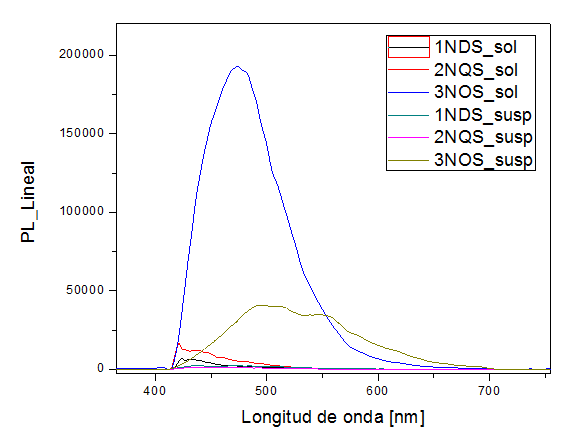
\includegraphics[width=0.8\textwidth]{resultados/sec1/emilinealtodas}
\caption{Espectros de emisi\'on lineal de 1NDS, 2NQS y 3NOS en soluci\'on y suspensi\'on de nanopart\'iculas}\label{eslia}
\end{subfigure}
\begin{subfigure}{\textwidth}
\centering
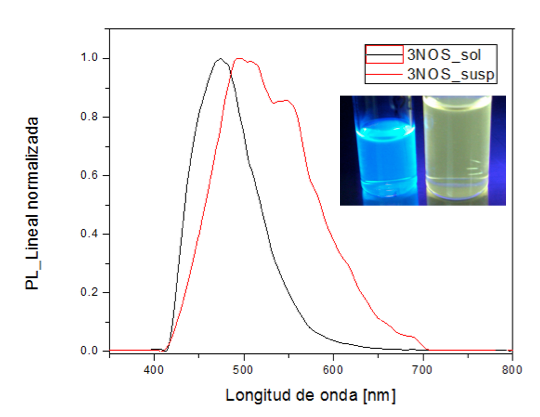
\includegraphics[width=0.8\textwidth]{resultados/sec1/emilinealnorm3N}
\caption{Espectros normalizados y fluorescencia visible de 3NOS en soluci\'on (azul) y suspensi\'on (amarilla) }\label{3nsolsusp}
\end{subfigure}
\caption{Espectros de emisi\'on lineal de 1NDS, 2NQS y 3NOS}
\label{ghghh}
\end{figure}

En comparaci\'on con el sistema octopolar, la emisi\'on (lineal y no lineal) de los sistemas dipolar y cuadrupolar fue muy escasa. Por ello \'unicamente fue de inter\'es medir varias veces la eficiencia cu\'antica de fluorescencia del sistema octopolar 3NOS, inicialmente en soluci\'on y suspensi\'on acuosa de nanopart\'iculas utilizando CTAB, nuevamente a una concentraci\'on de $6.25 \times 10^{-6}$; los valores obtenidos, utilizando la ecuaci\'on \ref{final}, se muestran en la tabla \ref{tablita}. 

Se realizaron tres y cinco mediciones de eficiencia cu\'antica de fluorescencia del sistema octopolar en soluci\'on y suspensi\'on respectivamente; adem\'as se realiz\'o una correcci\'on al valor de eficiencia promedio obtenido para la soluci\'on, debido a que la sensibilidad de respuesta del PMT no es la misma para todas las longitudes de onda. Cuando la fluorescencia de la muestra de inter\'es y de la referencia (Rodamina 6G) tienen longitudes de onda similares, el PMT responder\'a de la misma manera en ambas muestras; sin embargo, si la muestra y la referencia emiten a diferentes longitudes de onda, es necesario introducir un factor de correci\'on. En el caso de la soluci\'on octopolar dicho factor fue de 0.6.

\begin{table}[H]
\centering
\scalebox{0.82}{
\begin{tabular}{| c | c | c | c | c | c | c | c | r | }  %p{6.5cm} | c |
\hline
 3NOS           & $\Phi_1$	&$\Phi_2$ &$\Phi_3$&$\Phi_4$&$\Phi_5$& $\Phi_{Promedio}$&$\Phi_{Promedio}$ /correcci\'on PMT  \\ \hline   %\multicolumn{8}{|c|}
Soluci\'on &    0.457&	0.539& 0.341	& -	& -	&0.44& 0.26 \\ \hline
Suspensi\'on & 	0.129 &	 0.191& 0.094 & 0.225& 0.226	& 0.17&0.17 \\ \hline
\end{tabular} } 
\caption{ Valores obtenidos de eficiencia cu\'antica de fluorescencia $\Phi$ para el sistema octopolar  \label{tablita}}
\end{table}



